\documentclass{article}
\usepackage{tikz}

\begin{document}

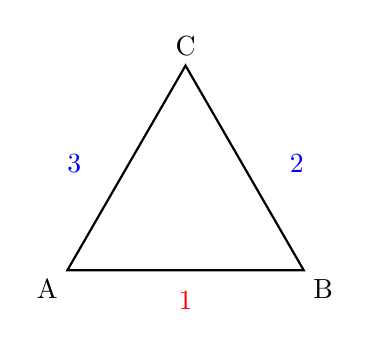
\begin{tikzpicture}[scale=1.5]

% Define colors
\definecolor{red}{RGB}{255,0,0}
\definecolor{blue}{RGB}{0,0,255}

% Draw the triangle
\draw[thick] (0,0) -- (2,0) -- (1,1.732) -- cycle;

% Label the vertices
\node at (0,0) [below left] {A};
\node at (2,0) [below right] {B};
\node at (1,1.732) [above] {C};

% Place numbers on the sides
\node at (1,-0.1) [below] {\textcolor{red}{1}};
\node at (1.8,0.9) [right] {\textcolor{blue}{2}};
\node at (0.2,0.9) [left] {\textcolor{blue}{3}};

\end{tikzpicture}

\end{document}